\section{Python: Interpolation Games}\label{sec:p6}

For $\phi_2$, we consider the equation $1/(z/8 + 3z/4 +z^{-1}/8)$:
\begin{align*}
	\frac{1}{\frac{1}{8}z + \frac{3}{4} + \frac{1}{8}z^{-1}}
	&= \frac{8}{z + 6 + z^-1} \\
	&= \frac{8}{z^{-1}(z^2 + 6z + 1)} \\
	&= \frac{8}{z^{-1}(z+3+2\sqrt{2})(z+3-2\sqrt{2})} \\
	&= \frac{8}{(1+(3+2\sqrt{2})z^{-1})(z+3-2\sqrt{2})} \\
	&= \frac{\frac{8}{3+2\sqrt{2}}}{(z^{-1}+3-2\sqrt{2})(z+3-2\sqrt{2})} \\
	&= \frac{\sqrt{\frac{8}{3+2\sqrt{2}}}}{z^{-1}+3-2\sqrt{2}} \cdot \frac{\sqrt{\frac{8}{3+2\sqrt{2}}}}{z+3-2\sqrt{2}}
\end{align*}
Therefore, we can choose $\mu = \sqrt{\frac{8}{3+2\sqrt{2}}}$ and $\gamma = 2\sqrt{2}-3$.

Figure \ref{fig:p6b} shows the interpolation results on the UIN and Figure \ref{fig:p6b} shows the results on 5 points inputted by mouse. The results of $\phi_0, \phi_1$, and $\phi_3$ are the same for the second figure.
\begin{figure}[htbp]
	\centering
	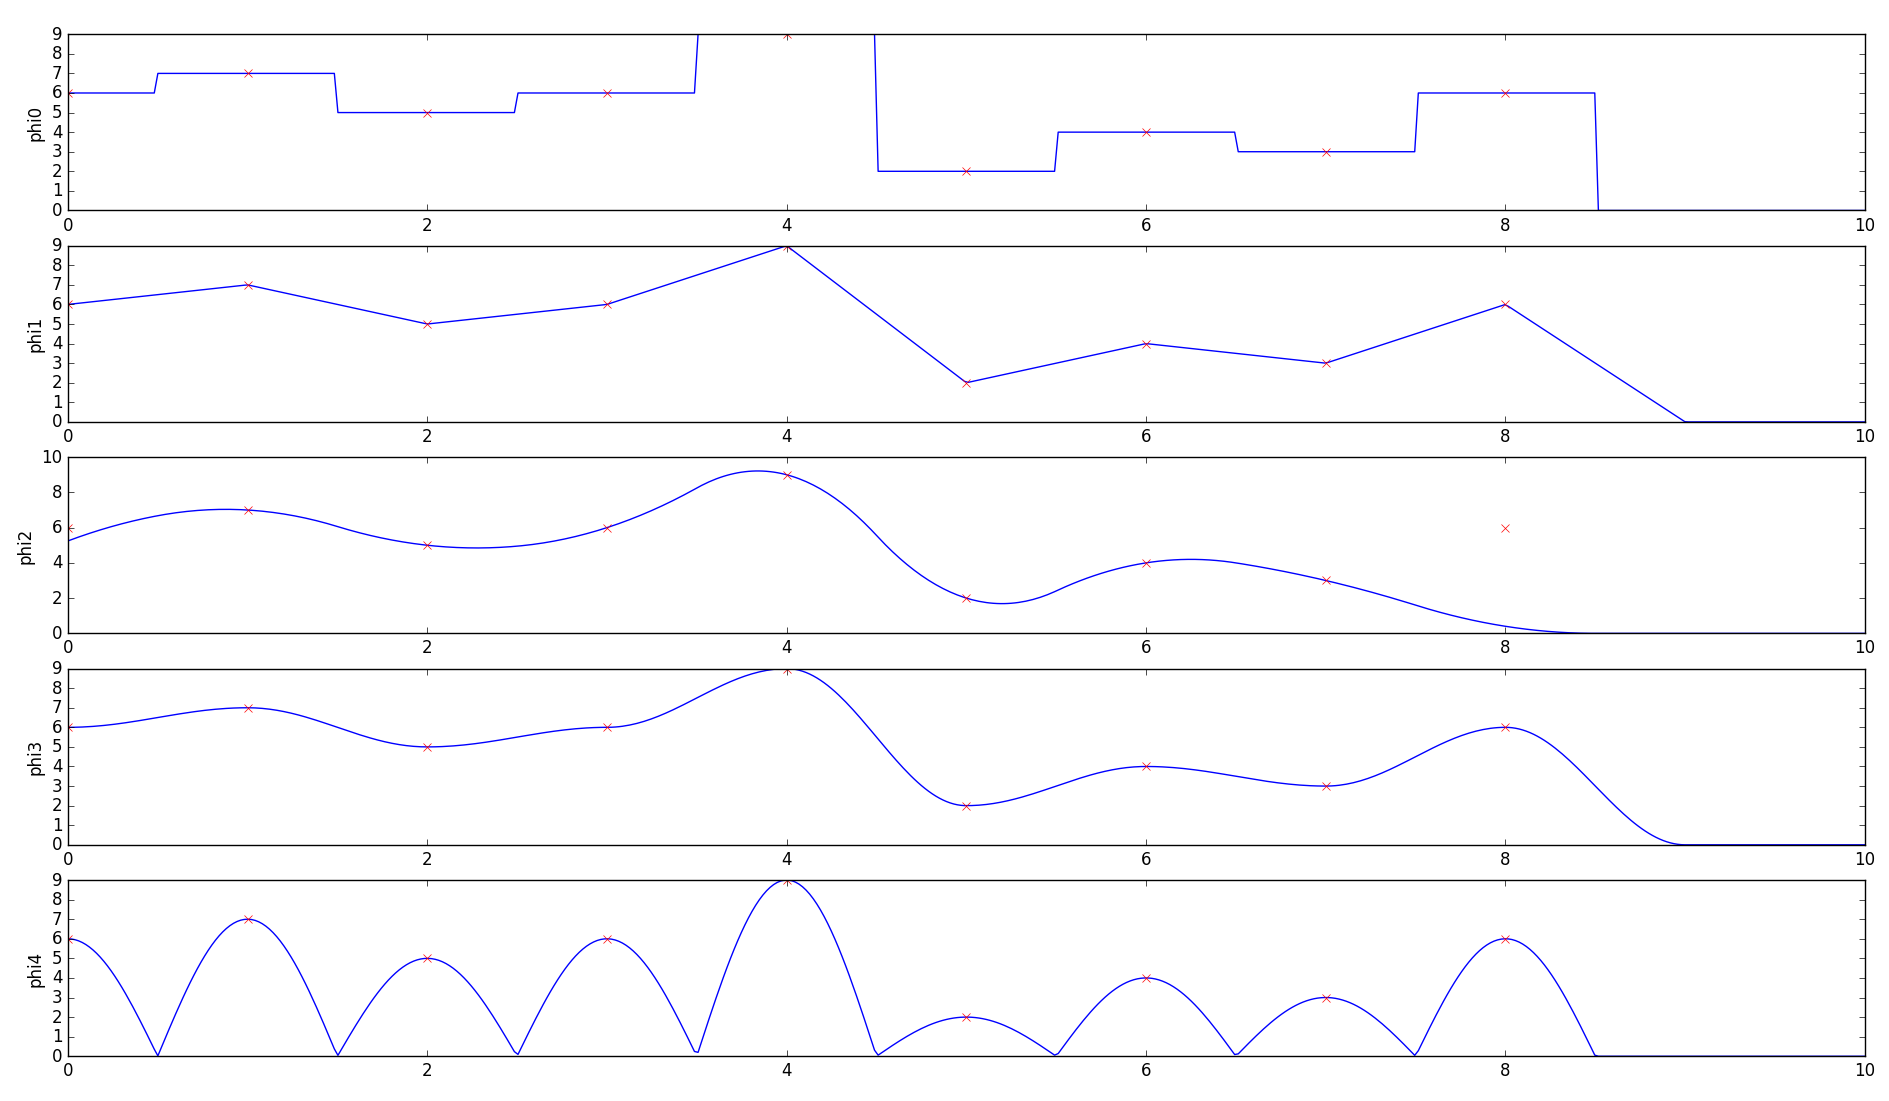
\includegraphics[width=\linewidth]{images/p6b}
	\caption{Interpolation results on the UIN}
	\label{fig:p6b}
\end{figure}

\begin{figure}[htbp]
	\centering
	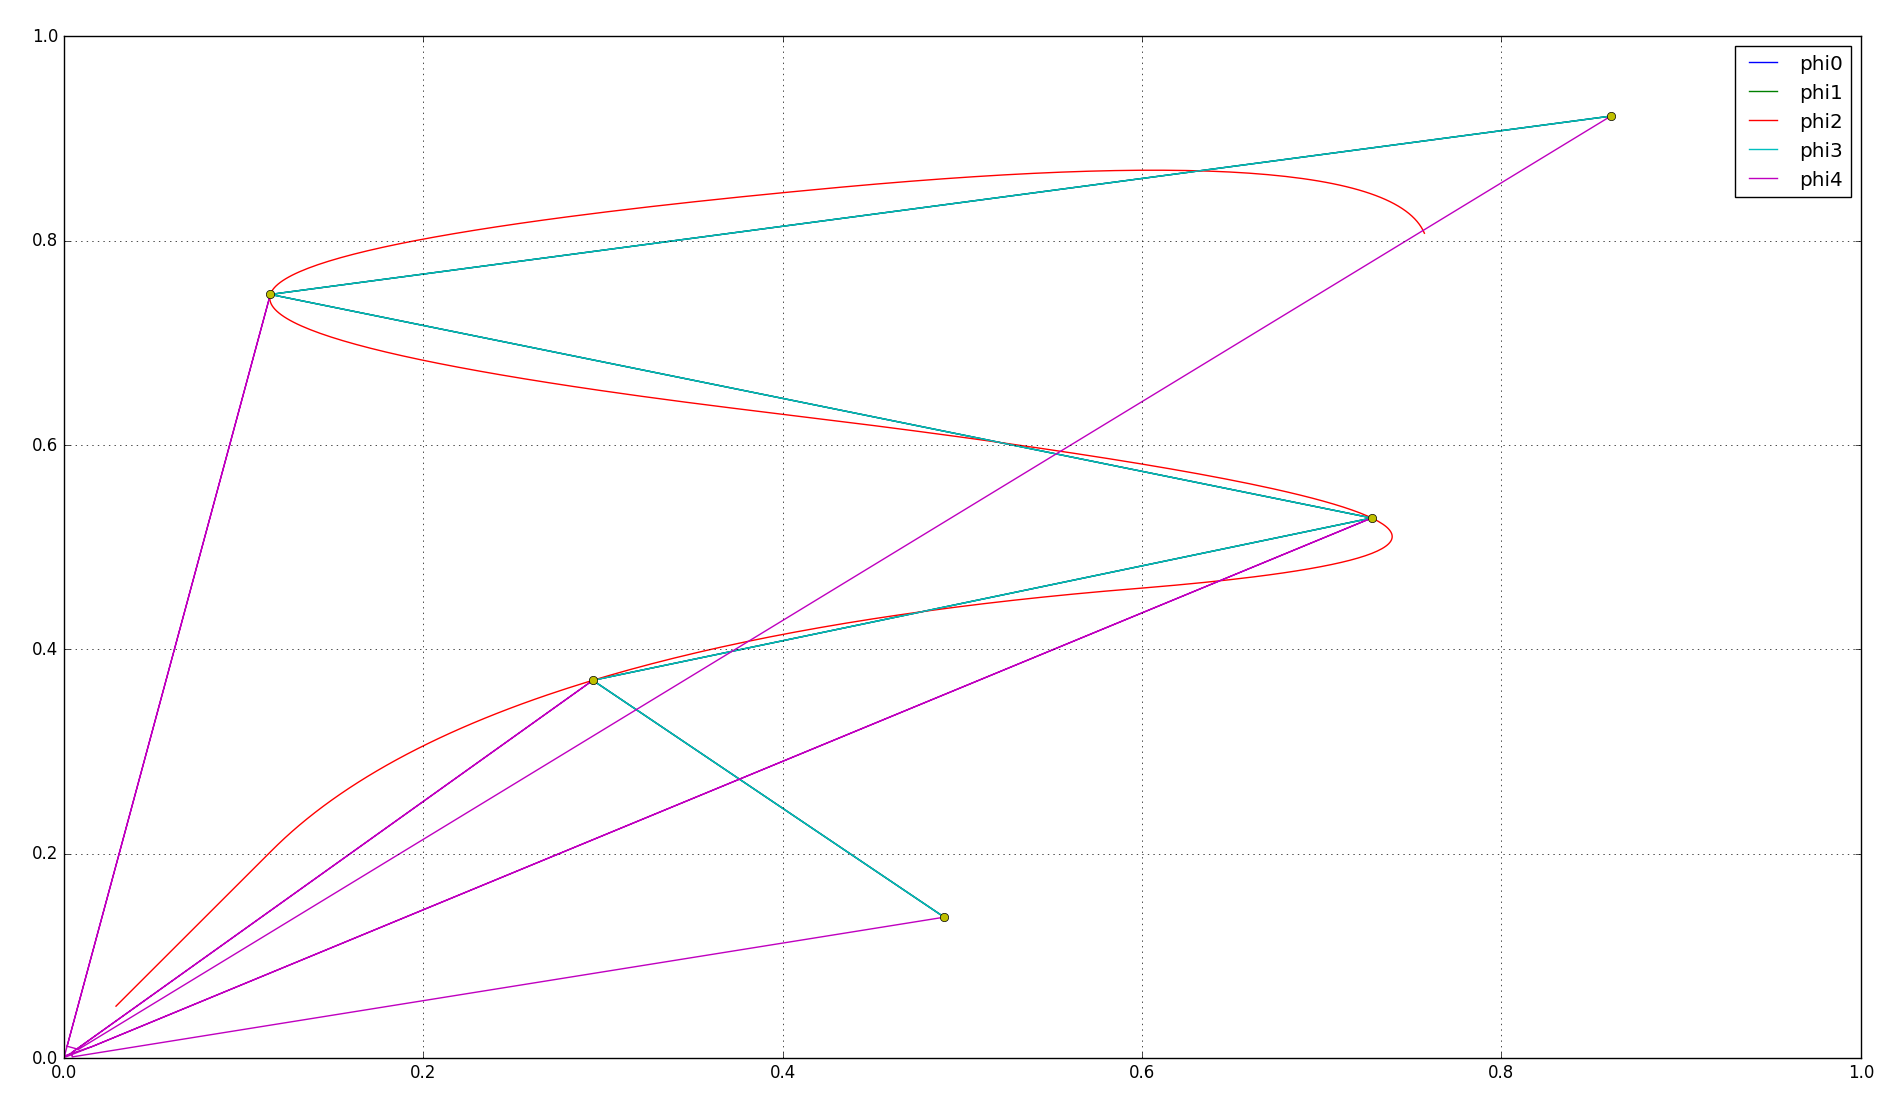
\includegraphics[width=\linewidth]{images/p6c}
	\caption{Interpolation results on 5 inputted points}
	\label{fig:p6c}
\end{figure}